\documentclass{article}
\usepackage{amsmath,amssymb}
\usepackage{graphicx}
\usepackage{bm}
\usepackage[numbers]{natbib}
\usepackage{color}

\title{The binary liquid model for gravity-driven microchannel simulations}
\date{\today}
\newcommand{\Ca}{\mathrm{Ca}}
\newcommand{\todo}[1]{{\color{red}#1}}
\begin{document}

\maketitle

\begin{abstract}
The motion towards exploration of nano- and microscale phenomena brings new
challenges to simulation tools. The continuous physics approach is limited on
those scales, and methods such as Molecular Dynamics (MD) or the Lattice
Boltzmann Method (LBM) become more appropriate. This work aims to
reproduce the gravity driven microchannel flow of a free surface liquid with the
help of the free-energy binary liquid lattice Boltzmann method. In the low capillary number
$\Ca$ regime, the flow is thoroughly described by Bretherton \cite{bretherton},
with the deposition film thickness proportional to $\Ca^{2/3}$. The binary
liquid model we use is a continuous-interface multiphase model, which presents
the question of how to properly resolve the interface to obtain proper correlations \todo{between what?}.
In this work we investigate how the binary liquid model parameters and the grid resolution
need to be adjusted to properly simulate microchannel flows.  The presented results
should be of interest for industrial applications and to researchers simulating
Bretherton phenomena.
\end{abstract}


\section{Introduction}
The Taylor/Bretherton \cite{bretherton} flow describes the flow of long bubbles in
microchannels. It was found that the front meniscus film width is proportional
to $\Ca^{2/3}$ for Capillary numbers less than $0.003$. While there are number
of works which simulate the Bretherton problem with the boundary value method
\cite{ingham-plates,heil-bretherton}, its simulation using diffusive interface methods
is difficult.  If the interfaec is spread over several grid nodes, the question of
proper film width resolution arises. While the discontinuous interface models
are good at simulating pheonomena in simple geometries, the continuous interface
methods are more flexible and capable of resolving problems involving coalescence
or droplet breakup. This work
concentrates on resolving the parameter range of the binary liquid lattice
Boltzmann method to validate it the Bretherton regime.

The lattice Boltzmann method has emerged as a successful method to simulate
a wide variety of phenomena including hydrodynamics \cite{yu}, thermal flows
\cite{karlin-minimalmodels}, microflows \cite{ansumali-small-knudsen},
ferrofluids \cite{kuzmin-aniso}, and multiphase flows
\cite{swift,Shan-chen:extended}. Thanks to its kinetic nature, LBM as a particle
method easily tackles complex geometries and the incorporation of
physical phenomena on the microscopic level, as is the case in multiphase models. Most
multiphase lattice Boltzmann models \cite{swift, Shan-chen:extended} resolve
the interface in a continuous way. Such a representation
brings issues with the film thickness resolution versus the interface
resolution. In other words, when it comes to the resolution of the film
thickness the diffusion \todo{diffusive?} interface should be resolved in such a way as to have
negligible effect on the physics of the film.

This work examines the binary liquid free-energy LB model \cite{swift}. The
model simulates two liquids with the assumption of uniform overall
density. Therefore, the question of how to simulate the Bretherton problem
where the two phases have two completely different densities (i.e. the two fluids
are liquid and gas) is of interest. However, in the case of the motion of a
liquid slug and a bubble in a capillary the governing factor is the capillary number
and the ratio of the viscosities, not of the densities, is the critical parameter.

The goal of this paper is to give an answer as to how to choose the
binary liquid model parameters, the viscosities ratio and the grid
resolution, in order to obtain correct Bretherton/Taylor film thickness.
The paper is organized as follows.  First, we briefly
explain the binary liquid lattice Boltzmann model and summarize the literature
for the Bretherton problem. Then, the parameters involved in the
simulation are examined and presented in the results section. The paper is
concluded with a summary of the main findings.

\section{Bretherton bubble flow}
Bretherton in his significant work \cite{bretherton} studied a long bubble
moving in a tube filled with liquid. It was found that the deposition film width
is proportional to $\Ca^{2/3}$ in the range of small capillary numbers. Later on
it was realized \cite{wong-films,wong-pressure} that the film deposition
is proportional to $\Ca^{2/3}$ only near the front meniscus and that the film width
varies throughout the bubble length for bubbles of finite length. Numerical
simulations \cite{giavedoni-numerical} and experimental studies
\cite{kreutzer-pressure-drop} showed as well a Reynolds number dependence, and
a deviation from the $\Ca^{2/3}$ rule for capillary numbers larger than $0.003$.
To be able to predict consistently the flow pattern for capillaries in
different ranges of parameters, simulations are developed and their codes
are typically validated with the small capillary numbers Bretherton problem.

There are a number of numerical methods which
were used for the simulation of the Taylor/Bretherton flow.
\citet{vanbaten-circular} studied the mass transfer and film
thickness for rising bubbles in a circular capillary.
\citet{kreutzer-pressure-drop} used the finite volume method to perform
simulations of a circular capillary for a number of different
Reynolds and capillary numbers. \citeauthor{wong-films} in
\cite{wong-films,wong-pressure} studied three-dimensional bubbles in
polygonal capillaries and showed the derivations of different shapes in the
slug crossections and menisci appearance.
\citet{heil-bretherton,ingham-plates} studied air finger propagation in
a two-dimensional channel for a range of Reynolds and capillary
numbers. \citet{giavedoni-numerical} performed crossvalidation of the
finite element solution developed by them with previously published results.
The solution is available for the circular and planar cases.

While the applicability of other methods is well established for the
simulation of the Bretherton/Taylor problem, this is not the case for
the lattice Boltzmann method. A thorough parameter study for this approach
has not yet been done to the best of the authors' knowledge.

One should acknowledge the works of \citet{pagonabarraga-fingers} on menisci
in thin films for fingering phenomena. \citet{sehgal-microchannel} performed lattice Boltzmann
simulations of two-dimensional channel flows for larger capillary numbers, and
the authors found discrepancies with the classical Bretherton theory, which
is limited to the low capillary number regime \cite{giavedoni-numerical}.

To resolve the interface on a fine level for capillary numbers less than
$0.003$ is computationally intensive even in the two-dimensional case
(the amount of memory necessary to perform the simulation is on the order
of tens or hundreds of gigabytes).  This work is therefore based on a
comparison with the already established results, which were themselves
validated for the Bretherton bubble flow.  In this paper, we present
recipes for the initialization of the simulations and discuss optimal
parameter ranges for the binary liquid LB model.

\section{Lattice Boltzmann binary liquid model}
The lattice Boltzmann equation (LBE) operates on a rectangular grid representing the
physical domain. It utilizes
probability distribution functions (also known as particle populations)
containing information about
macroscopic variables, such as fluid density and momentum. LBE consists of
two parts: a local collision step, and a propagation step which transports
information from one node to another in certain
directions specified by the discretized velocity set.
The LBE is typically implementated as follows:
\begin{equation}
\label{standard:implementation}
\begin{aligned}
&f_i^{*}(\bm{x},t)=\omega f_i^{eq}(\bm{x},t)-(1-\omega) f_i(\bm{x},t) +
F_i,&&\text{ collision step}\\
&f_i(\bm{x}+\bm{c_i},t+1)=f_i^{*}(\bm{x},t),&&\text{ propagation step}, 
\end{aligned}
\end{equation}
where $F_i$ is the external force population. The binary fluid LB model is
based on a free-energy functional \cite{swift,landau}, and operates with two
sets of populations: one to track the pressure and velocity fields, and the
other to represent the phase field.

The model we use in this work is a two-dimensional nine-velocity (D2Q9) model,
with equilibrium populations \cite{pooley-contact}:
\begin{equation}
\begin{aligned}
&f_i^{eq}=w_i 
\biggl(3
p_0 - k \phi \Delta \phi
+\frac{u_{\alpha}c_{i\alpha}}{c_s^2}+\frac{Q_{i\alpha\beta}u_{\alpha } u_ {
\beta}}{2 c_s^4}\biggr), i=1\div8\\
&f_0^{eq}=\rho-\sum_{i\neq0}{f_i^{eq}}\\
&g_i^{eq}=w_i\left(\Gamma \mu + \frac{\phi c_{i\alpha} u_{i\alpha}}{c_s^2}+\phi^m
\frac{Q_{i\alpha\beta}u_{\alpha}u_{\beta}}{2 c_s^4}\right), i=1\div8 \\
&g_0^{eq}=\phi-\sum_{i\neq0}{g_i^{eq}}\quad,
\end{aligned}
\end{equation}
where $\Gamma$ is the mobility parameter; the chemical potential
$\mu=-A\phi+A\phi^3-k\Delta\phi$; $k$ is related to the surface
tension; $A$ is a parameter of the free-energy model  The bulk pressure
is expressed as $p_0=c_s^2 \rho +A (-0.5 \phi^2+0.75 \phi^4)$. 
Parameters speficic to the D2Q9 grid are the weights
$w_i=\left\{\frac{4}{9},\frac{1}{9},\frac{1}{9},\frac{1}{9},\frac{1}{9},
\frac{1}{36},\frac{1}{36},\frac{1}{36},\frac{1}{36}\right\}$, and the tensor
$Q_{i\alpha\beta}=c_{i\alpha} c_{i\beta} - c_s^2 \delta_{\alpha\beta}$ with
the sound speed parameter $c_s^2=1/3$.  The weights related to the
inclusion of the surface tension coefficient into the equations are as follows:
$w^{xx}_{1-2}=w^{yy}_{3-4}=1/3$, $w^{xx}_{3-4}=w^{yy}_{1-2}=-1/6$,
$w^{xx}_{5-8}=w^{yy}_{5-8}=-1/24$, $w^{xy}_{1-4}=0$, $w^{xy}_{5-6}=1/4$ and
$w^{xy}_{7-8}=-1/4$. The system can be shown to restore the macroscopic
fluid equations as:
\begin{equation}
\begin{aligned}
&\partial_t \rho+ \partial_{\alpha} \rho u_{\alpha}=0\\
&\rho\left(\partial_t+u_{\beta}\partial_{\beta}\right) u_{\alpha}=
-\partial_{\alpha}P_{\alpha \beta} +
\nu\partial_{\beta}\left(\partial_{\alpha}u_{\beta}+\partial_{\beta} u_{\alpha}
+ \frac{1}{3}\partial_{\gamma} u_{\gamma} \delta_{\alpha\beta}\right)\\
&\partial_t \phi + \partial_{\alpha} \phi u_{\alpha}=M \Delta \mu,
\end{aligned}
\label{binary:fluid:system}
\end{equation}
where $\nu=c_s^2 (\tau-1/2)$ is the viscosity and
$M=\Gamma(\tau_{\phi}-1/2)$ is the mobility parameter. The system allows the separation of the liquid
phase with $\phi=1$ and a so-called gas phase with $\phi=-1$. The
relaxation time is taken to depend linearly on the relaxation
times $\tau_{\mathrm{gas}}$ and $\tau_{\mathrm{liq}}$:
$\tau=\tau_{\mathrm{gas}}+\frac{\phi+1}{2}\tau_{\mathrm{liq}}$.
The surface tension in the framework of the binary liquid model is $\sqrt{8 k A}{9}$ \todo{is this right?  should the 9 be in the
denominator?  is not, perhaps put before the root?}.

\section{Lattice Boltzmann benchmark}
To properly simulate and to compare simulation results with the data
published in the literature, one needs to design a numerical benchmark addressing
the following challenges for the lattice Boltzmann method:
\begin{itemize}
 \item The diffusive nature of the interface in the multiphase model should not
influence the film width results. This is obviously achieved only for certain
resolutions of the interface in comparison with the film width.
 \item Spurious currents arising from surface tension discretization
can influence mass transfer in the thin film, thereby comoromising the
overall solution. The bubble should therefore be long enough to decrease the
influence of spurious currents.
 \item The wettability coefficient which in principle can control the
dynamic angle and the menisci appearance \cite{pagonabarraga-finger} should not
influence the overall solution.
 \item The free-energy model examined in the work is single density, two
viscosities model. The classical Bretherton problem is a free-interface problem
where the film thickness is established by itself. The viscosity ratio should
be large, as indicated in \cite{pagonabarraga-fingers}, however no studies
address this issue. \todo{what's the conclusion of the impact of this issue to our paper then?}
  \item The Bretherton problem addresses bubble flow driven by a pressure
difference, not a body force.  It is however relatively difficult to impose a
pressure difference in the framework of the binary liquid model, as two
simultaneous boundary conditions with the associated gradients and laplacians are required.
This kind of pressure boundary conditions for the binary liquid model is currently
under development, and preliminary results show that the differences between
pressure difference flows and flows driven by a body force are small as far as the film
deposition thickness is concerned.  In this work we limit ourselves to the study
of body force driven flows, because of their simplicity and better numerical stability.
 \item Most simulations are done for a circular channel,
which is quite difficult to address in terms of lattice Boltzmann free energy
framework where one needs to calculate Laplacians near the boundaries.
Although one can apply certain finite difference stencils
\cite{arnold-boundary,hunt-boundary} developed specifically for curved boundaries,
the analysis of error introduced by the boundary conditions becomes an issue.
Our benchmark is therefore done is for an axis-symmetric case. \todo{since this paper
is about a 2d flow, which we already said in the intro, what is the point of discussing
curve boundaries which are only an issue in 3d?}
\end{itemize}
Given all the concerns and challenges, the suggested lattice Boltzmann framework
is a two-dimensional flow driven by a body force.  An analytical
solution to this problem is to the best of our knowledge not yet known.
Though some authors \cite{sehgal-microchannel} use the gravity driven model to
validate the Bretherton film thickness, the latter should be used with caution
since the velocity of the bubble is different from the fluid velocity and the
bubble shape
is different in the front and rear menisci. \citet{wong-films} indicated that the
film width for polygonal capillaries
changes from $\Ca^{1/2}$ on distances $x\propto \Ca^{-1}$ to $\Ca^{2/3}$ for
distances $x \gg \Ca^{-1}$. Therefore, for a bubble to have a formed shape in
the  front meniscus we chose the bubble length to be $5$ channel heights. The
channel length is taken  as $3$ bubble lengths (or $15$ channel heights)
to minimize the influence of one bubble on another,
because of the periodicity of boundary conditions.
Figure \ref{fig:benchmark:sketch} represents a sketch of the geometry
used in the benchmark.
\begin{figure}
%\includegraphics[width=0.97\textwidth]{}
\caption{{\color{red} Ask Sasha to help here. The benchmark sketch.}
\label{fig:benchmark:sketch}}
\end{figure}


\section{Results}
\subsection{The nondimensionalization and initialization procedure}
We now intrduce the procedure of nondimensionalization, as well as
the initialization techniques we used to be able to predict parameters necessary for
simulation. The capillary number governs the interface thickness and is defined as:
\begin{equation}
Ca=\frac{U_{\mathrm{bubble}} \mu_{\mathrm{liq}}}{\gamma},
\end{equation}
where $\mu_{\mathrm{liq}}$ is the liquid viscosity, and $\gamma$ is the surface tension. The
bubble velocity $U_{\mathrm{bubble}}$ is taken in the center of the bubble where the film
thickness is examined.
While parameters such as $\mu_{\mathrm{liq}}$, $\gamma$ and the capillary number $\Ca$ are given
or defined through the model parameters, the velocity $U_{\mathrm{bubble}}$ is not.
In the simulation we approximately match the velocity with the
Poiseuille profile center velocity, which is given by the equation:
\begin{equation}
\begin{aligned}
U_{\mathrm{bubble}} \approx U_{\mathrm{liq}}=\frac{H^2}{8
\mu_{\mathrm{liq}}}\frac{\mathrm{d}P}{\mathrm{d}x}\\
U_{\mathrm{bubble}}\approx
\frac{{N_y}^2}{\frac{8}{6}(\tau_{\mathrm{liq}}-\frac{1}{2})}\frac{\mathrm{d}P}{\mathrm{d}
x } ,
\end{aligned}
\end{equation}
By taking the Poiseuille profile one can estimate the body force through the
capillary number and grid resolution:
\begin{equation}
\label{poiseuille:velocity:center}
\begin{aligned}
&\frac{\mathrm{d}P}{\mathrm{d}x}=\frac{8}{{N_y}^2}\gamma Ca.
\end{aligned}
\end{equation}
In practice, we iterate adjusting the body force value until both the desired velocity and the
capillary numbe are achieved.

After one calculates the parameters necessary to run a simulation, one needs to
initialize the macroscopic fields and particle populations.
The velocity is initialized with $0$ everywhere. Populations are initialized
with the equilibrium values for the binary liquid model, including all the phase
gradients and Laplacians. The liquid phase is initialized with $\phi = 1$ and the
gas phase is initialized with $\phi = -1$. Though the initialization film thickness
is not involved in the final result for the front meniscus (see Fig.
\ref{fig:different:initialization:widths}) we keep the initialized film
thickness as close as possible to the already obtained numerical film
thickness values \cite{giavedoni-numerical}. This is done to minimize
the simulation time, as starting far away from the steady-state requies
additional time for the relaxation.
\begin{figure}
\includegraphics*[bb=-20 360 620 430,width=0.97\textwidth]
{Figures/Init/initbegin12.eps}
\includegraphics*[bb=-20 360 620 430,
width=0.97\textwidth]{Figures/Init/initbegin16.eps}
\includegraphics*[bb=-20 360 620 430,
width=0.97\textwidth]{Figures/Init/initbegin20.eps}
\includegraphics*[bb=-20 360 620
430,width=0.97\textwidth]{Figures/Init/initfinish12.eps}\\
\includegraphics*[bb=-20 360 620
430,width=0.97\textwidth]{Figures/Init/initfinish16.eps}\\
\includegraphics*[bb=-20 360 620
430,width=0.97\textwidth]{Figures/Init/initfinish20.eps}\\
\caption{The phase plots for different bubble widths as
$H_{\mathrm{eff}}-12$,$H_{\mathrm{eff}}-16$ and
$H_{\mathrm{eff}}-20$. The grid for the simulation is $102 \times 1501$. The phase
profiles were obtained after $2\cdot10^5$ time steps. One can see that even if the
system is initialized with different bubble volumes, the bubbles always relaxate
to a shape where the film thickness is conserved. For the given parameters the
interface thickness is $0.0615$, $0.0611$, $0.0605$.
\label{fig:different:initialization:widths}}
\end{figure}

Here, two different examples are presented that can quantitatively show the
initialization procedure for quite different capillary numbers. In these
examples we use $k=0.04$ and $A=0.04$ as optimal binary liquid model parameters.
That explicitly implies the surface tension to be $\sqrt{\frac{8 k
A}{9}}=0.0377$ and the characteristic length of the interface
$5\sqrt{\frac{k}{A}}=5$ lattice boltzmann units. For the sake of simplicity and
stability the relaxation times for liquid and gas phases are taken as
$\tau_{\mathrm{liq}}=2.5$ and $\tau_{\mathrm{gas}}=0.7$, which corresponds
to a gas-liquid viscosity ratio of $10$.
\begin{description}
 \item[I \bm{$Ca=0.005$}]
  The film width for such small Capillary numbers \cite{bretherton} is
given by the equation:
  \begin{equation}
  \frac{h_{\infty}}{H}=1.3375 \Ca^{2/3}=0.03899,
  \end{equation}
  where we assume that $2 H$ or $N_y$ is the channel width in lattice units.

\todo{Therefore one needs to resolve the interface which is around $2$ percent of
the  whole channel width with, for instance $8$ lattice units, where $5$ lattice
units occupies the interface width for given. Note that the interface occupies
$62.5$ percent of the interface. -- these two sentences need to be rewritten for clarity}  Therefore the channel
  width is $400$ lattice units.

  We take the bubble length as $5$ channel widths
  and the distance between bubbles is $2$ bubble lengths. This gives a
grid size of $400 \times 6000$. In terms of computer memory
requirements, the calculations with double precision accuracy demand:
\begin{equation}
\begin{aligned}
&2\text{ sets of populations } \times \,\, 8\,\, \text{bytes per population
} \times \,\, 9 \text{ number of
populations}\\
&\times\,400\,\times\,6000\approx 345 \mathrm{MB}. 
\end{aligned}
\end{equation}
Even with this naive assumption for the $50$ percent resolution of the film
width in comparison with the interface width, one can get the memory
requirement of $345 \mathrm{MB}$. 

After resolving the interface one can  calculate the
  velocity from the capillary number as:
  \begin{equation}
  U_{\mathrm{bubble}}=0.005 \frac{\gamma}{\mu_{\mathrm{slug}}}=0.005
\frac{0.0377}{0.66666}=2.82 \cdot10^{-4},
  \end{equation}
  where $\mu_{\mathrm{slug}}=1/3 (2.5-0.5)=0.6666$.
  This velocity implies the following pressure gradient calculated from the
  Poiseuille flow solution: \todo{maybe add a ref, to this eq. from the previous section?}
  \begin{equation}
  \begin{aligned}
  &U_{\mathrm{bubble}}=\frac{H^2}{8\mu} \frac{\mathrm{d}P}{\mathrm{d}x}=\frac{N_y^2}{8/3
  (\tau_{\mathrm{liq}}-1/2)}\frac{\mathrm{d}P}{\mathrm{d}x}\\
  &\frac{\mathrm{d}P}{\mathrm{d}x}=\frac{8}{N_y^2}\gamma Ca
  \end{aligned}
  \end{equation}
  The pressure gradient is then:
  \begin{equation}
  \begin{aligned}
  \frac{\mathrm{d}P}{\mathrm{d}x}=9.42 \cdot 10^{-9}.
  \end{aligned}
  \end{equation}
  Note that in the case of large grids  height resolution is directly
involved in calculation of the physical time step :since:
\begin{equation}
\Delta t =\frac{U_{\mathrm{LBM}}}{U_{\mathrm{phys}}} \Delta x ,
\end{equation}
where for example the real velocities in the physical world can reach
approximately $1$ m/s and physical channel height up to $1$ mm. In this case one
can easily approximate the physical time step:
\begin{equation}
\Delta t = 7.05 \cdot 10^{-10} \,\mathrm{s}
\end{equation}
which is quote small. A typical simulation needs approximately
$100000-300000$ time steps to come to the steady state solution giving the
physical time simulation around $10^{-5}-10^{-4}\,\mathrm{s}$, which is
probably not enough to find the desired correlations. \todo{correlations between what?}

 \item[II $\bm{Ca=0.05}$] 
   The parameters in the previous subsection imply very long
simulations. Bretherton delivered his solution for the range of Capillary number
less than
  $0.005$. However, a lot of simulations devoted to the Bretherton/Taylor
flow extended it to the range of Capillary numbers greater than
$0.005$, and to different Reynolds numbers. One can refer to figures
  \ref{fig:giavedoni:planar} and \ref{fig:heil:planar} taken from the work of
  \citet{giavedoni-numerical,heil-bretherton}, who crossvalidated their
  simulations with Bretherton and each other. Even though the LBM can simulate
flows with small capillary numbers, i.e. less than $0.005$, the simulation time
is relatively long. Therefore, we focus our work on the simulations of
\citet{giavedoni-numerical} who crossvalidated
results for all ranges of capillary numbers.  Our intention is
  to show proper physics behavior for moderate parameters
which
  can be easily and quickly validated on a computer.
  One can see from Fig. \ref{fig:heil:planar} that the width for the
  Capillary number $0.05$ ranges from $0.12$ to $0.15$, while the Reynolds
  number ranges from $0$ to $300$.

  The film width for such small Capillary numbers is taken from
  \ref{fig:heil:planar}, and for Reynolds number $40$ equals $0.12$. We want to
  resolve $6\%$ of whole channel width with $12$ lattice units, where $5$
lattice units are related to the interface resolution.  Therefore the channel
  width is $200$ lattice units. We take the bubble length as $5$ channel widths
  with distance between slugs being $2$ bubble lengths \todo{this I think is the 3rd
  time this particular geometry is mentioned in this paper, perhaps just skip it in this place?}. That gives
the grid size of $200 \times 3000$. The velocity can be
calculated from the Capillary number as:
  \begin{equation}
  U_{\mathrm{bubble}}=0.05 \frac{\gamma}{\mu_{\mathrm{liq}}}=0.05 \frac{0.037712}{0.6666}=2.82\cdot
  10^{-3}.
  \end{equation}
  The velocity implies the following pressure gradient calculated from the
  Poiseuille flow solution:
  \begin{equation}
  \begin{aligned}
  &\frac{\mathrm{d}P}{\mathrm{d}x}=\frac{8}{N_y^2}\gamma Ca=3.77\cdot10^{-7}.
  \end{aligned}
  \end{equation}
  Our approach to the initial conditions is  to take values from the previously performed
numerical simulations and to calculate the grid sizes from them, matching the
body force gradient through the solution of Poiseuille flow.

\end{description}
\begin{figure}
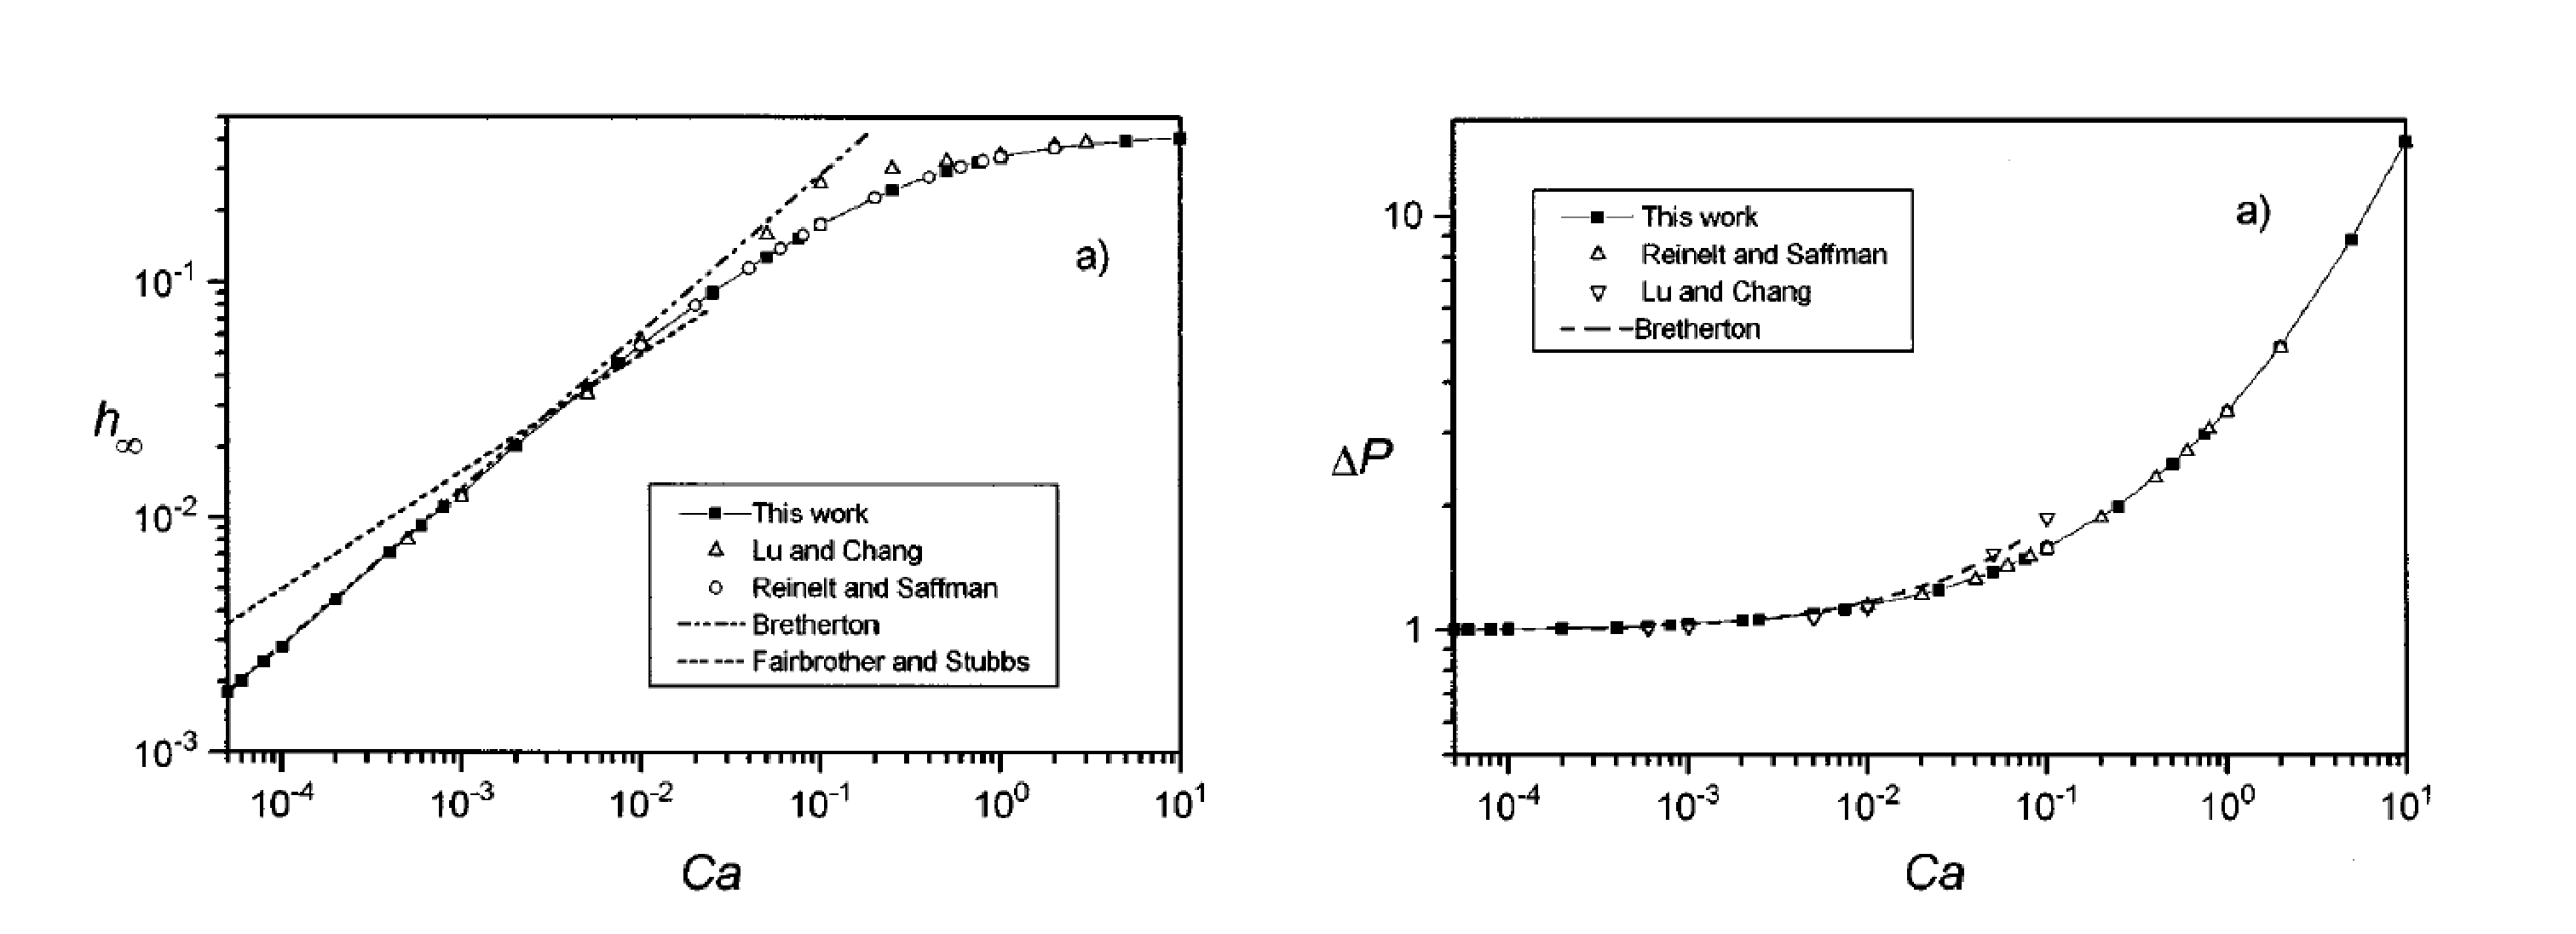
\includegraphics[width=0.97\textwidth]{Figures/giavedoni_planar.eps}
\caption{\citet{giavedoni-numerical} gathered results across the
literature for different Capillary numbers \label{fig:giavedoni:planar}}
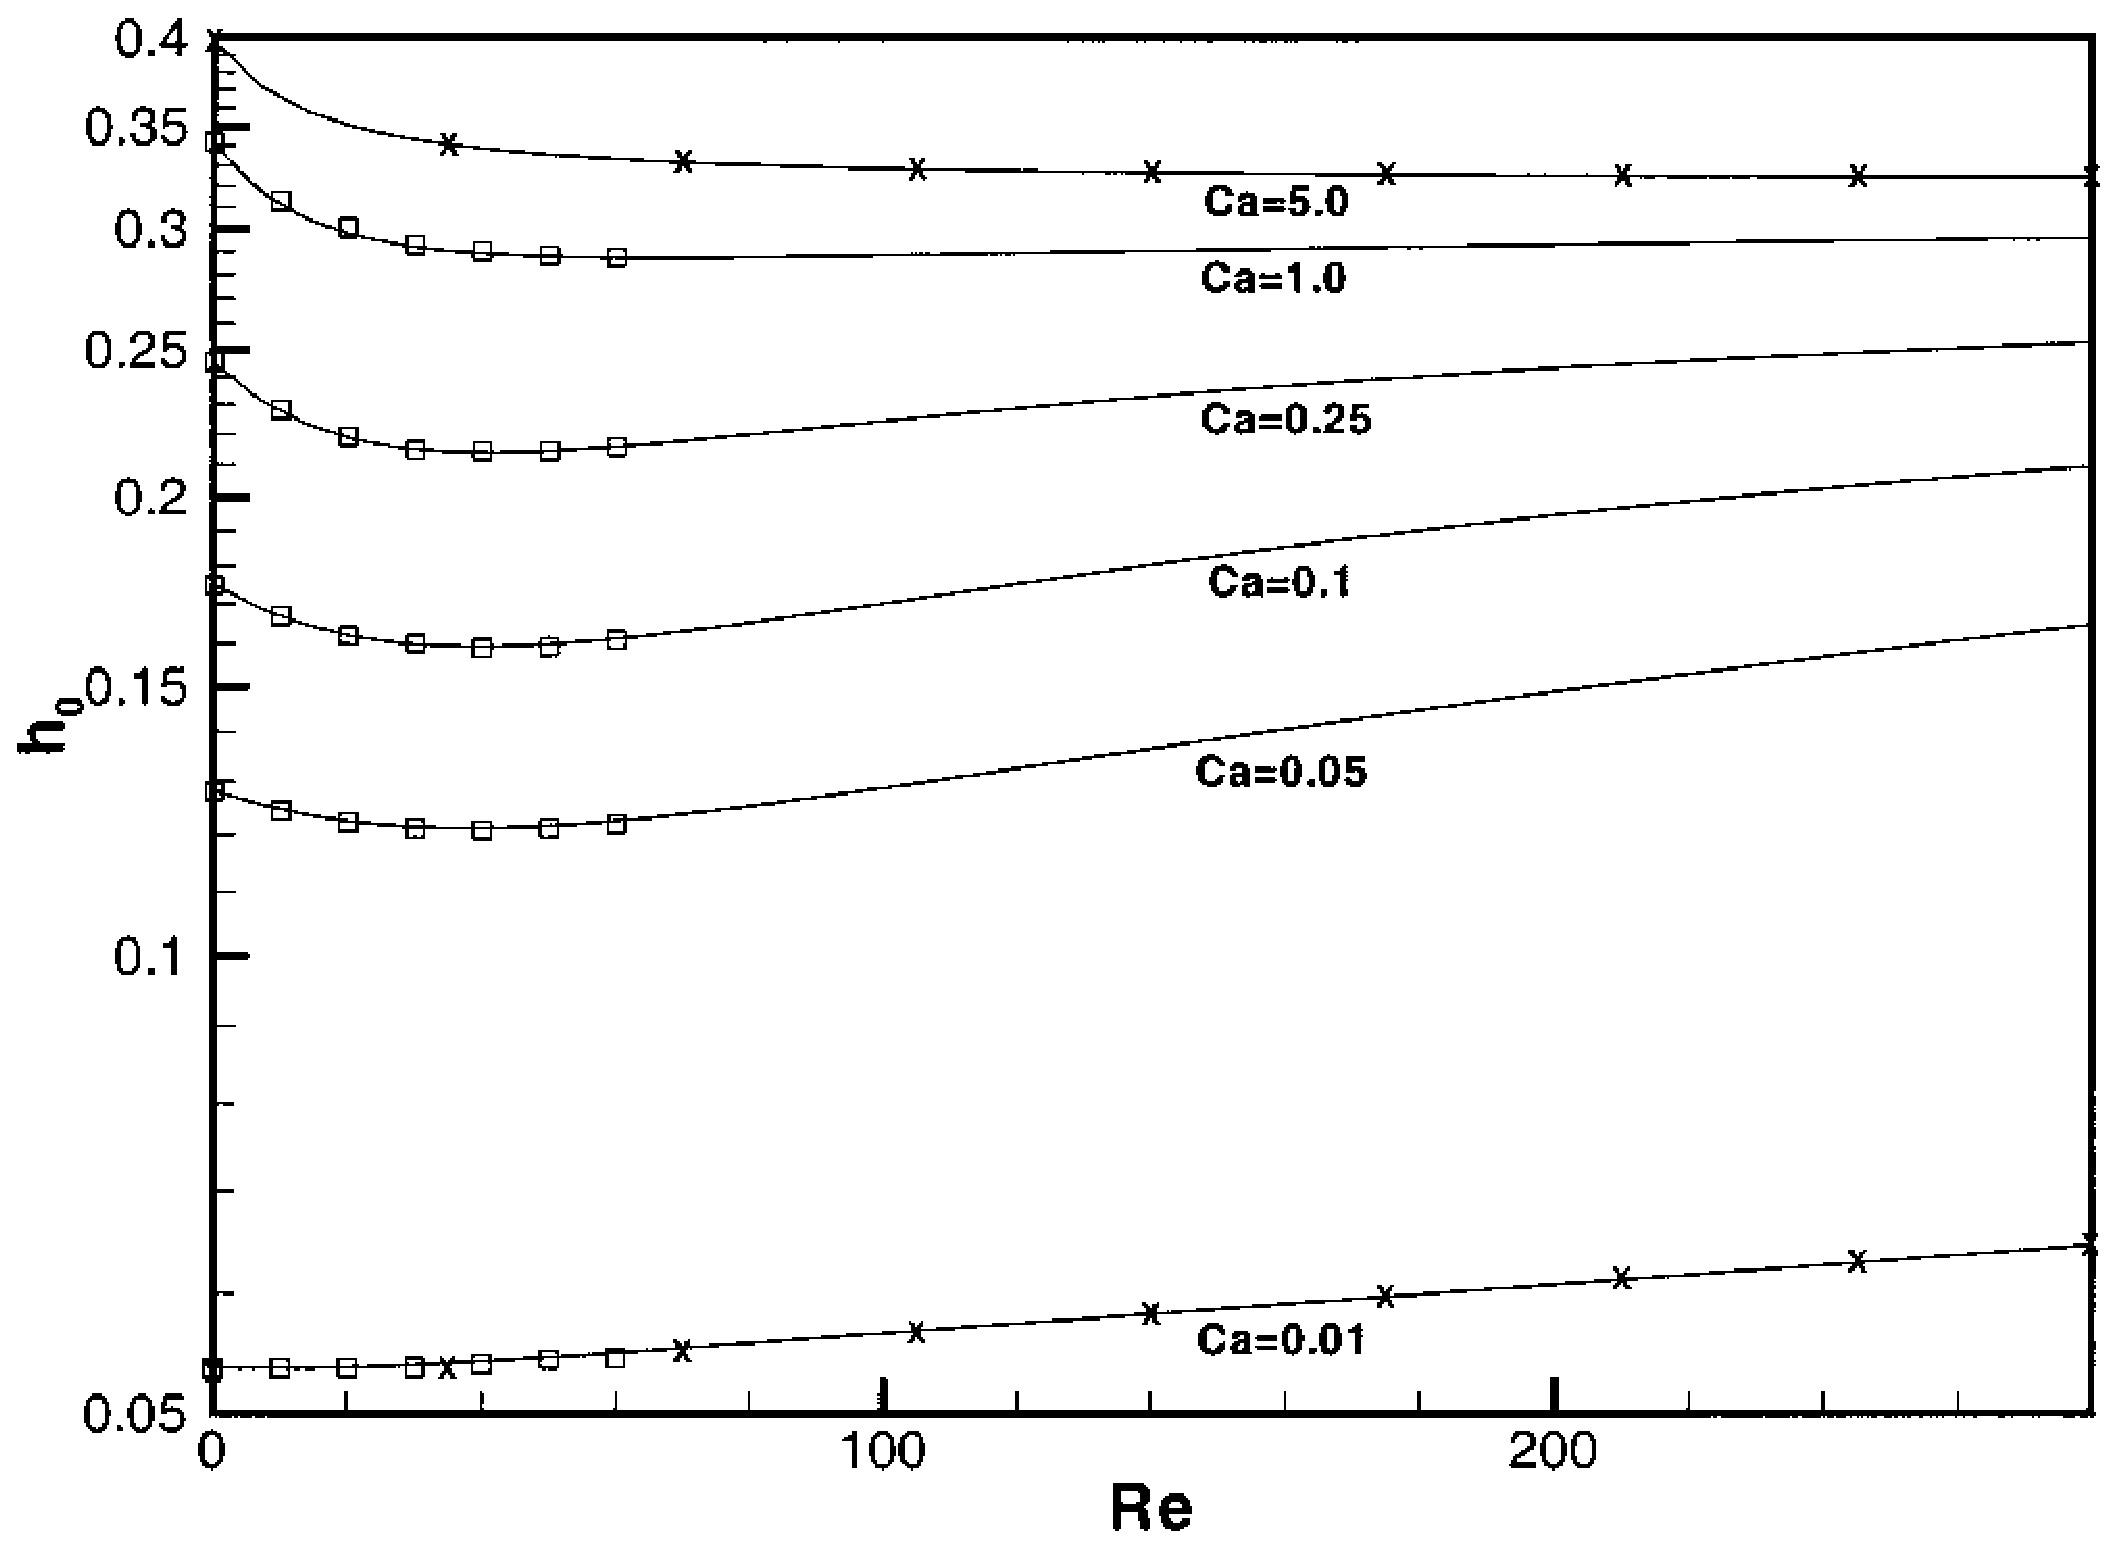
\includegraphics[width=0.97\textwidth]{Figures/heil-planar.eps}
\caption{\citet{heil-bretherton} performed simulations for different ranges of
Capillary numbers and Reynolds numbers. \label{fig:heil:planar}}
\end{figure}
Note that we base the initialization techniques on correlations for the
capillary number and the body force. However, in the binary liquid framework
those correlations are only approximate. The biggest assumption lies
in calculating the body force from the Poiseuille velocity profile.
In reality, the less viscous bubble will have a slippage
factor and its velocity is larger than the surrounding liquid velocity. By
plugging in the obtained velocity back to the capillary number equation the
larger capillary number can be obtained. While we present the initialization
tips, in practice one needs to take the bubble velocity from the simulations and
recalculate all the necessary characteristics or in other words adjust the
forcing to obtain the desired velocity/capillary number.

\subsection{Grid refinement}
To properly estimate the interface resolution one needs to study the convergence
of the results of a function of the grid resolution. To do that, all parameters are held fixed,
including the bubble velocity, the capillary number, an only the grid
resolution is changed. Our goal is to know exactly the ratio of the interface width to the
film thickness where results are not dependant on the grid resolution.

We illustrate the procedure in more detail for the capillary number
$0.05$. As it was pointed out earlier, the film thickness in that case is $6$ percent.
Note that in the case of the half-way bounce-back walls \todo{the bounce-back
proceduce was not described earlier in this paper} which are used in the
simulations one needs to calculate the film thickness as:
\begin{equation}
\delta=(\phi_0-0.5)/(N_y-2),
\end{equation}
where $\phi_0$ is the grid coordinate where phase field is $0$, $N_y-2$
is related to the effective channel height. Note that it is a big
simplification to impose the boundary in the middle beetween the bounce-back
node and the fluid node which give rise to the viscosity dependent location of
the wall \cite{ginzburg-multireflection}. In the case of $\delta=0.06$ the
initial grid size is $N_y=102$, which gives the horizontal grid size as $N_x-1=15(N_y-2)=1500$.
The bubble is initialized as a rectangular box with coordinates
$y=7\dots N_y-8$, $x=\frac{N_x}{3}\dots \frac{2 N_x}{3}$ and phase
$\phi_{\mathrm{bubble}}=-1$. All other nodes are initialized with the phase field
$\phi=1$. The force gradient can be estimated through the Poiseuille
profile formula, Eq.~\ref{poiseuille:velocity:center}, and it equals
$1.508 \cdot 10^{-6}$.

After choosing the reference parameters, the grid refinement procedure
needs to keep the macroscopic parameters constant.  Therefore the simulations
were performed with grid numbers $N_y=102,127,152,177,202,227$, corresponding to the
effective channels widths  $H_{\mathrm{eff}}=100,125,150,175,200,225$,
$N_x=1501,1876,2251,2626,3001,3376=15
H_{\mathrm{eff}}+1$. It is easy to check
that keeping all liquid viscosities the same yields the following quantity to
be independent of grid size
$H_{\mathrm{eff}}^2\frac{\mathrm{d}P}{\mathrm{d}x}=(N_y-2)^2\frac{\mathrm{d}P}{\mathrm{d}
x } = \mathrm{const}$. We performed a number of simulations for the prescribed grids.
The unified scaled profiles are shown in Fig. \ref{fig:grid:profiles}. One can
see the visual results converge for $H_{\mathrm{eff}}\geq 175$. The calculated widths
are $0.0606$,$0.0618$,$0.0617$,$0.0629$,$0.0624$,$0.0624$. We accept the
convergent results for grids larger than $H_{\mathrm{eff}}=175$. However, one can see
that with proper initialization techniques, large enough time and the wall
wettability, results are different only in the 3rd digit even for
underresolved film widths. To calculate how well the interface thickness is
resolved, the ratio of the interface thickness to the film width thickness is calculated. The
interface itself occupies approximately $5 \xi$, where
$\xi=\sqrt{k/A}=1$. Let us calculate the interface width ratio to the film
thickness as
$5\xi/H_{\mathrm{film}}$: $0.824$, $0.646$,  $0.539$, $0.453$,
$0.400$, $0.355$. Therefore, one needs to
resolve the interface as $40-50$ percent of the
expected film width for simulations to be convergent. We further examine the
velocities in the center of the bubble to calculate the Capillary number. The
calculated numbers are $0.0041$, $0.0041$,$0.0040$,$0.0040$,$0.0041$,$0.0039$.
This corresponds to the average capillary number of $0.07$, which is slightly
larger than the expected capillary number. The corresponding error can be
attributed to the density and viscosity ratios which are much larger in the
Bretherton problem.
\begin{figure}
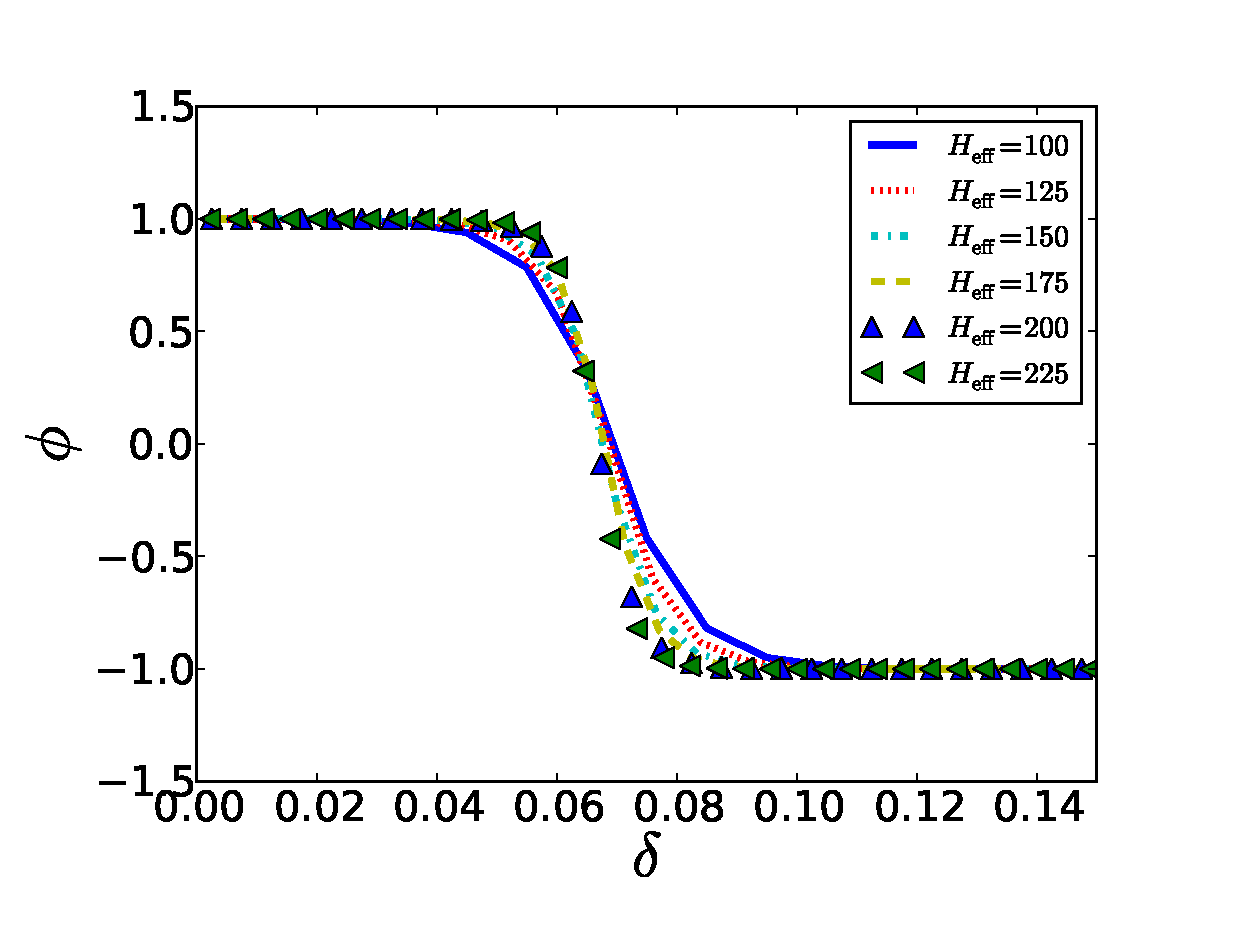
\includegraphics[width=0.97\textwidth]{Figures/Grid/norm_grid_profs.eps}
\caption{Grid-refined profiles for the effictive
channel widths
$H_{\mathrm{eff}}=100,125,150,175,200,225$.One can see
convergent results even for the underresolved film
thickness.\label{fig:grid:profiles}}
\end{figure}

\subsection{The influence of the wall gradient}
The simulation results should not depend on the wall wettability. Wettability is defined
through the phase gradient \cite{pooley-contact}, $\partial_n \phi$.  We took a large
enough grid resolution in order for simulations to be consistent -- the grid size was
$177 \times 2626$ and the initial film width was
$12$ lattice boltzmann units, which corresponds to the predicted film thickness.
We examined $11$ different values for the wall
gradient ranging from $-1$ to $1$. The results are consistent among all the
wall gradients given that the interface is resolved in the right way. For the
given wall gradients the values of interface thickness values are
$0.0633$,$0.0634$,$0.0634$,$0.0634$,$0.0634$,$0.0634$,$0.0633$,$0.0632$,
$0.0631$. The results are different in 4th digit. For the wall gradients $0.8$
and $1.0$ the
simulations are unstable. One can see the simulated profiles in Fig.
\ref{fig:gradients:profiles}. Negative values of the phase gradient are
preferable, since the phase of the liquid adjacent to the wall has the value of $1$.
The phase values near the wall are above $1$ and do not interact
with the bubble which has phase value $-1$.  In case of positive
gradients the values near the wall are below $1$, and the gradient profile can
fuse with the values of the gas phase as, giving rise to an unphysical wall stickyness.
\begin{figure}
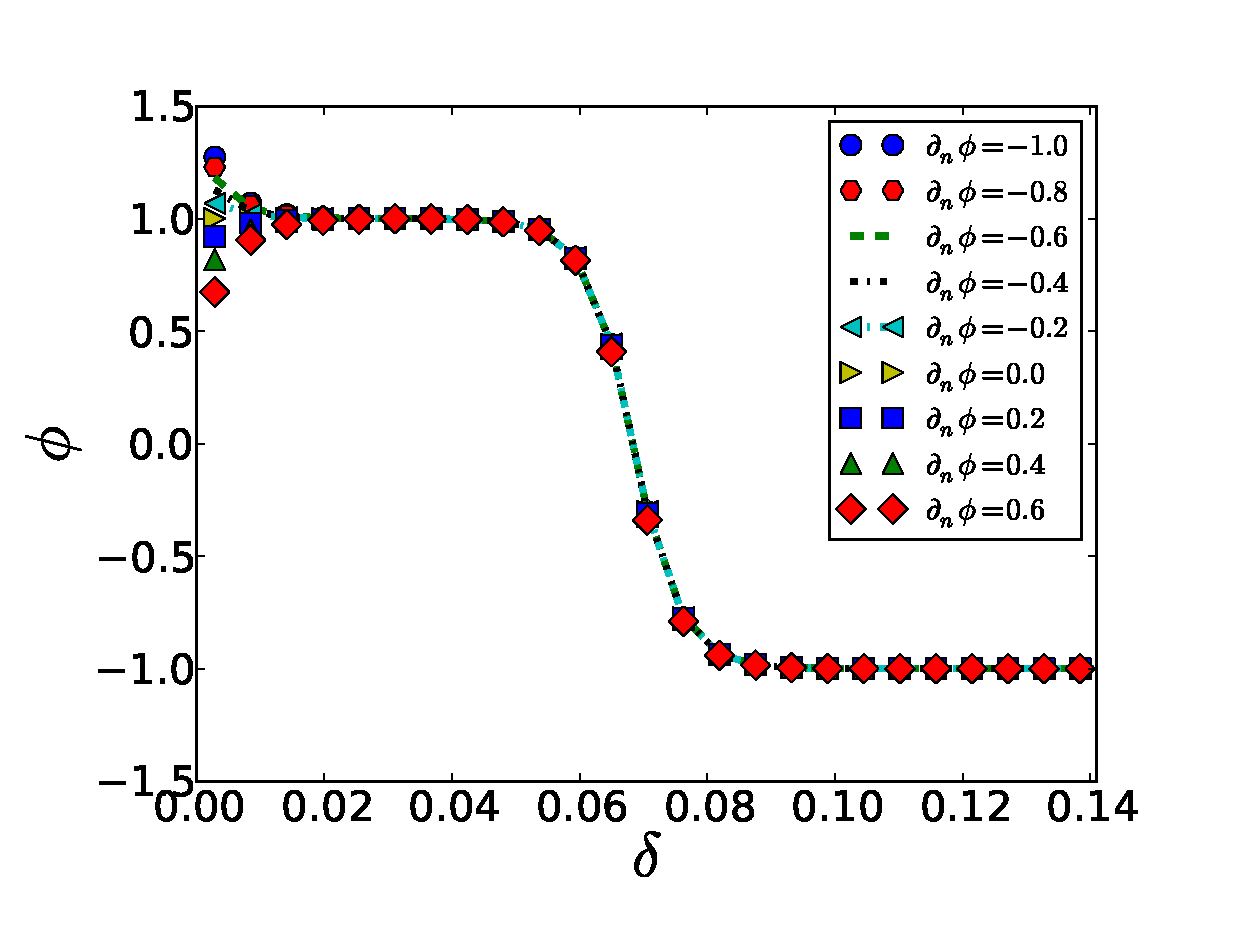
\includegraphics[width=0.97\textwidth]{Figures/Wall/phase_grad_profiles.eps}
\caption{Phase profiles for different wall gradients. One can see that if the width
is properly resolved then the wettability of the wall does affect the film thickness.
\label{fig:gradients:profiles}
}
\end{figure}
Another question which arises is the influence of the wall gradient on the bubble velocity and the
corresponding capillary number. The shear stress controlled by the wall phase gradient changes the
effective velocity near the wall, thus changing the bubble velocity as well.
One can see that if the film thickness is resolved properly the influence of the wall gradient can
be neglected. Fig. \ref{fig:velocities:wall:gradient} shows the center bubble velocity for different
gradients. The average relative error around the mean velocity is $0.1\%$.
\begin{figure}
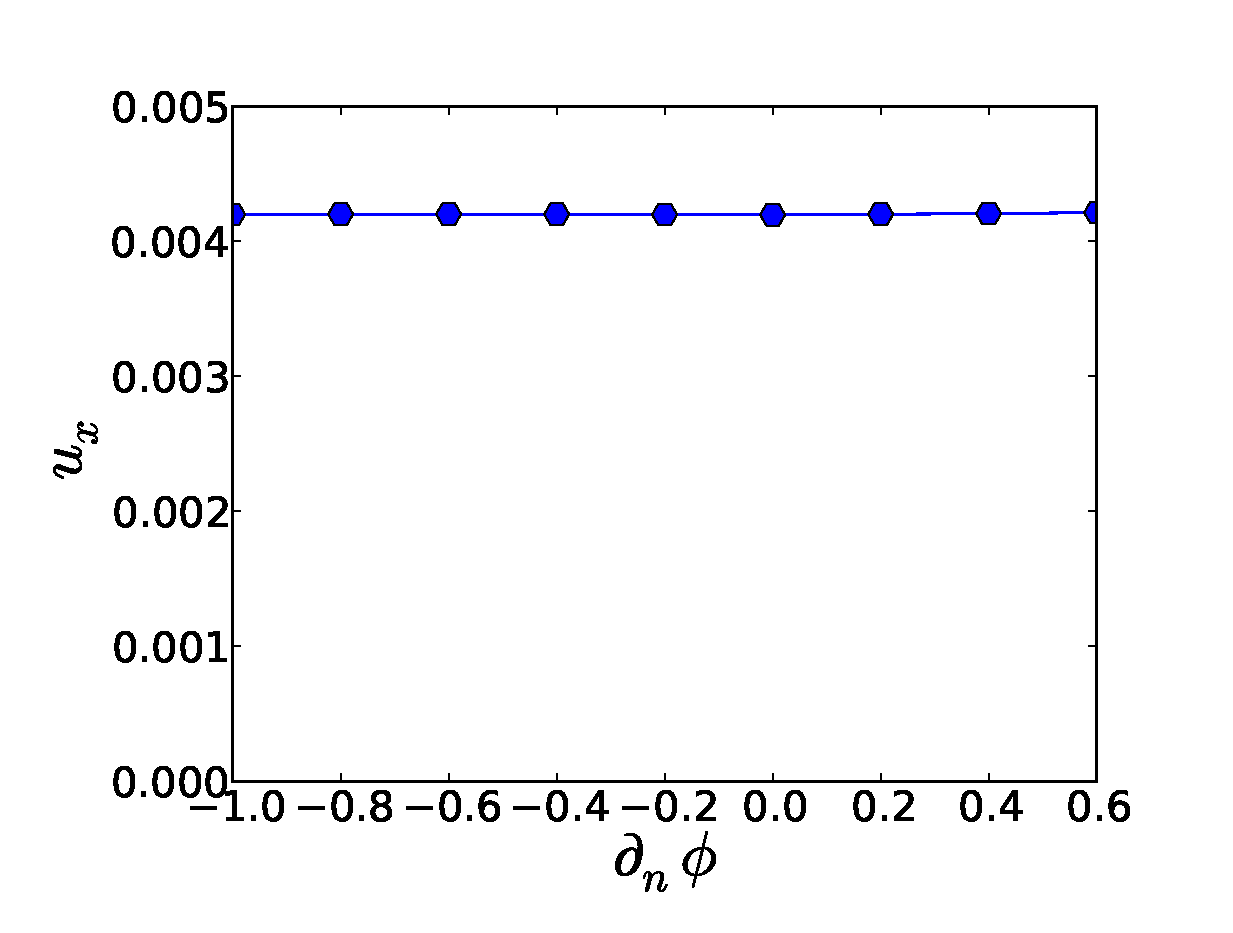
\includegraphics[width=0.97\textwidth]{Figures/Wall/velocities_grad_profiles.eps}
\caption{The center bubble velocity versus the phase gradient. One can neglect the influence of
the wall once the film is properly resolved.
\label{fig:velocities:wall:gradient}
}
\end{figure}

\subsection{Capillary number region}
The purpose of this section is to validate the correlations of
\citet{giavedoni-numerical}, Fig. \ref{fig:giavedoni:planar}, and
\citet{heil-bretherton}, Fig. \ref{fig:heil:planar}, for a range of capillary
numbers. Because of limited computational resources, we skip the
small capillary numbers and compare the film thickness over the capillary number
range from $0.03$ to $0.8$, which is a computationally reasonable task.  For the
benchmark
results we
suggest the following Capillary numbers:
\begin{equation}
0.03,0.05,0.08,0.1,0.2,0.4,0.6,0.8\, .
\end{equation}
The corresponding approximate film widths from \cite{giavedoni-numerical} are as
follows:
\begin{equation}
0.04,0.06,0.08,0.1,0.12,0.13,0.15\,.
\end{equation}
To perform numerical simulations we refer
to the grid refinement section where we established that the interface width should be
at most $50$ percent of the interface width.  We therefore choose the grid to be
$202 \times 3001$. $5$ lattice Boltzmann units do not occupy more than $60$
percent of the effective width. Because the simulation get unstable with
smaller grids and larger gradients, all the capillary number simulations were
performed on the chosen grid. To properly initialize the force gradient, the
proportionality law was utilized. The forcing
$6 \cdot 10^{-6}/16$ was chosen to obtain the predicted capillary
number $0.005$. The forcing for other grids can be obtained using
simple correlations:
\begin{equation}
\begin{aligned}
&Ca_{\mathrm{lit}} \propto U_{\mathrm{bubble}}\\
&U_{\mathrm{bubble}} \propto \frac{\mathrm{d}P}{\mathrm{d}x} N_y^2\\
&Ca_{\mathrm{lit}} \propto \frac{\mathrm{d}P}{\mathrm{d} x} N_y^2 \text{ or }\\
&\frac{\mathrm{d}P}{\mathrm{d} x} \propto \frac{\Ca_{\mathrm{lit}}}{N_y^2},
\end{aligned}
\end{equation}
where the index ,,lit'' stands for the predicted capillary number
\cite{giavedoni-numerical,heil-bretherton}. The grid number $N_y$ is not
involved because all simulations are conducted on the same grid.
The pressure gradient can be obtained through the capillary numbers
ratio:
\begin{equation}
\frac{\mathrm{d}P}{\mathrm{d} x}=6 \cdot 10^{-6}/16 \frac{Ca_{\mathrm{lit}}}{0.05}
\end{equation}
The film width is initialized through the capillary numbers ratio as well:
\begin{equation*}
w=12 \frac{Ca_{\mathrm{lit}}}{0.05}
\end{equation*}
The results were obtained after $2\cdot10^5$ steps. The following film thicknesses were
calculated: $0.042$,$0.066$, $0.085$, $0.077$, $0.123$, $0.153$, $0.164$, $0.173$ with
the corresponding bubble center velocities $0.0022$, $0.0041$, $0.0068$, $0.0055$,
$0.0185$, $0.0388$, $0.0592$, $0.0782$. Based on the obtained center velocities,
the capillary numbers are calculated as
$0.039$,$0.072$,$0.120$,$0.098$,$0.328$,$0.686$,$1.046$,$1.383$. These
capillary numbers are overpredicted but the obtained lengths are overpredicted
as well due to the improper body force imposement \todo{what is improper about? do you refer
to the fact that the Poiseuille should not be sued here?}.  We extracted data from
\cite{giavedoni-numerical,heil-bretherton} and compared it the results of our
simulations, which is shown in Fig. \ref{fig:capillary:comparison}.
\begin{figure}
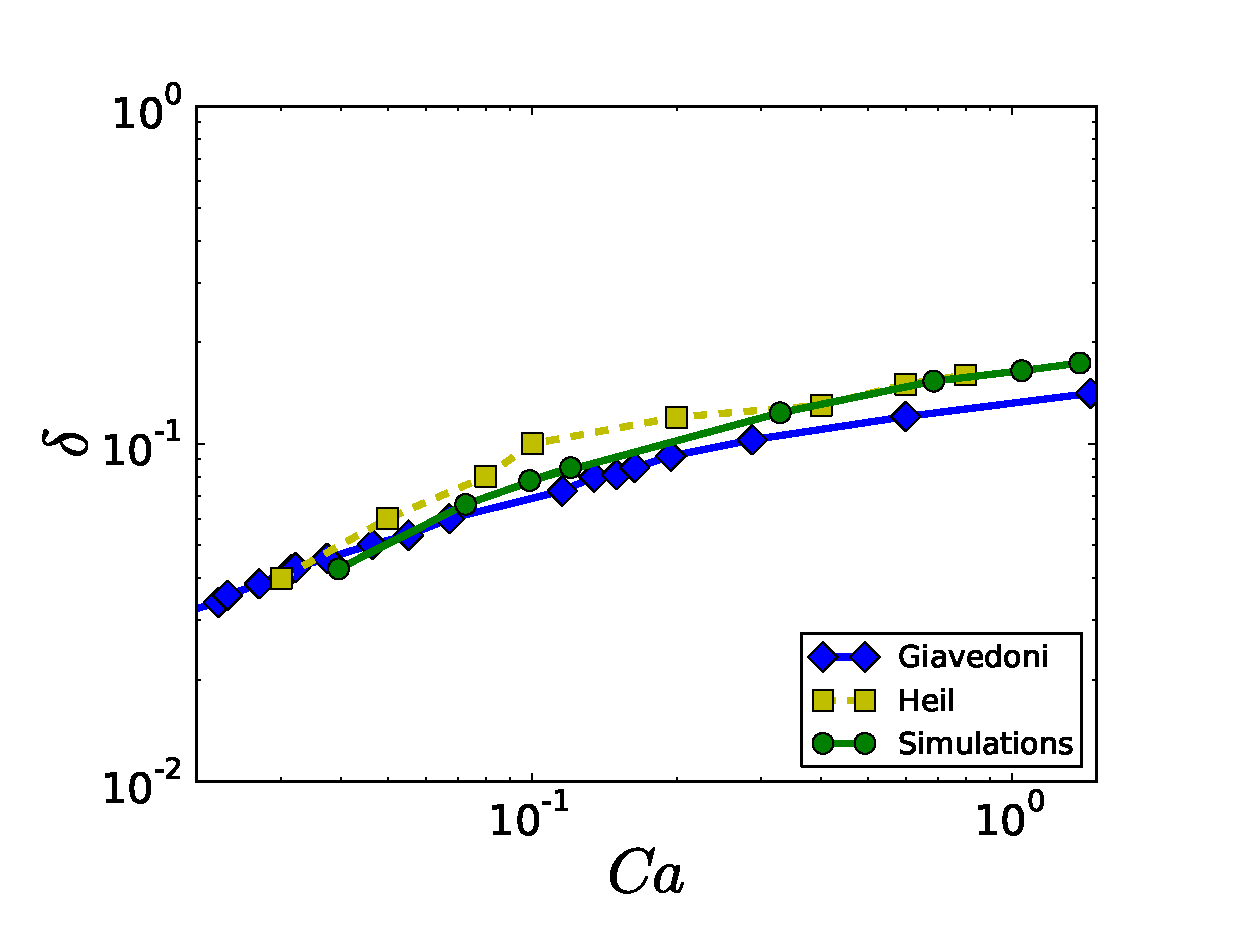
\includegraphics[width=0.97\textwidth]{Figures/Capillary/capillaries_comparison.eps}
\caption{A comparison between simulation results and results from
\cite{giavedoni-numerical} and \cite{heil-bretherton}. One can see a
reasonable agreement. The plots depict the film thickness as a function of the
the capillary number.\label{fig:capillary:comparison}}
\end{figure}


\subsection{The film variation over the bubble}

Next, we investigated the qualitative variation of the film thickness over the bubble length.
Though there are simulations for the bubble length for the two-dimensional case, due to
the presentation of data it is hard to extract numerical values from the plots. One can see bubble lengths
variations for the two-dimensional simulations for the range of capillary numbers in Fig.
\ref{fig:sehgal:bubble:length}.
\begin{figure}
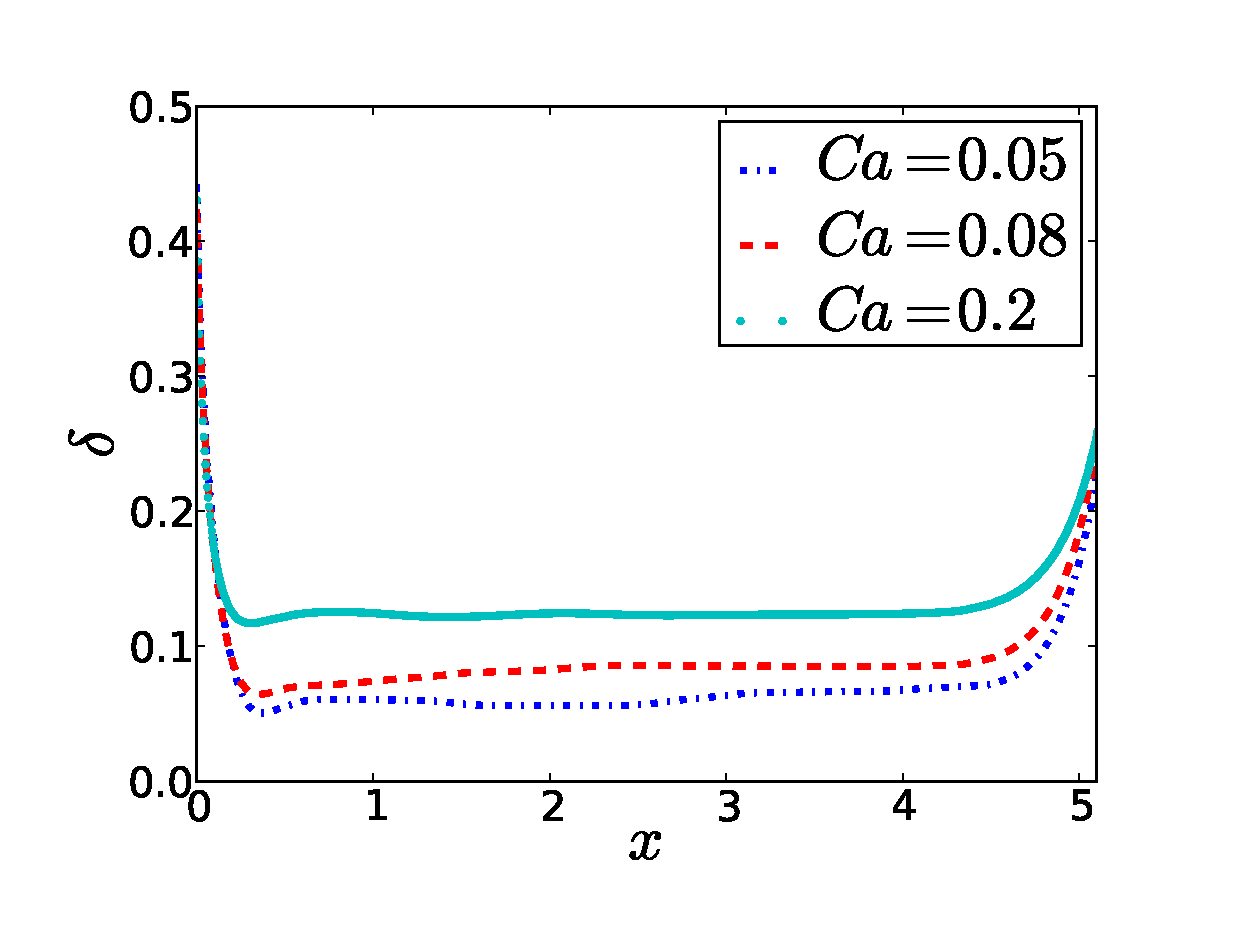
\includegraphics[width=0.47\textwidth]{Figures/Bubble/bubble_length.eps}\hfill
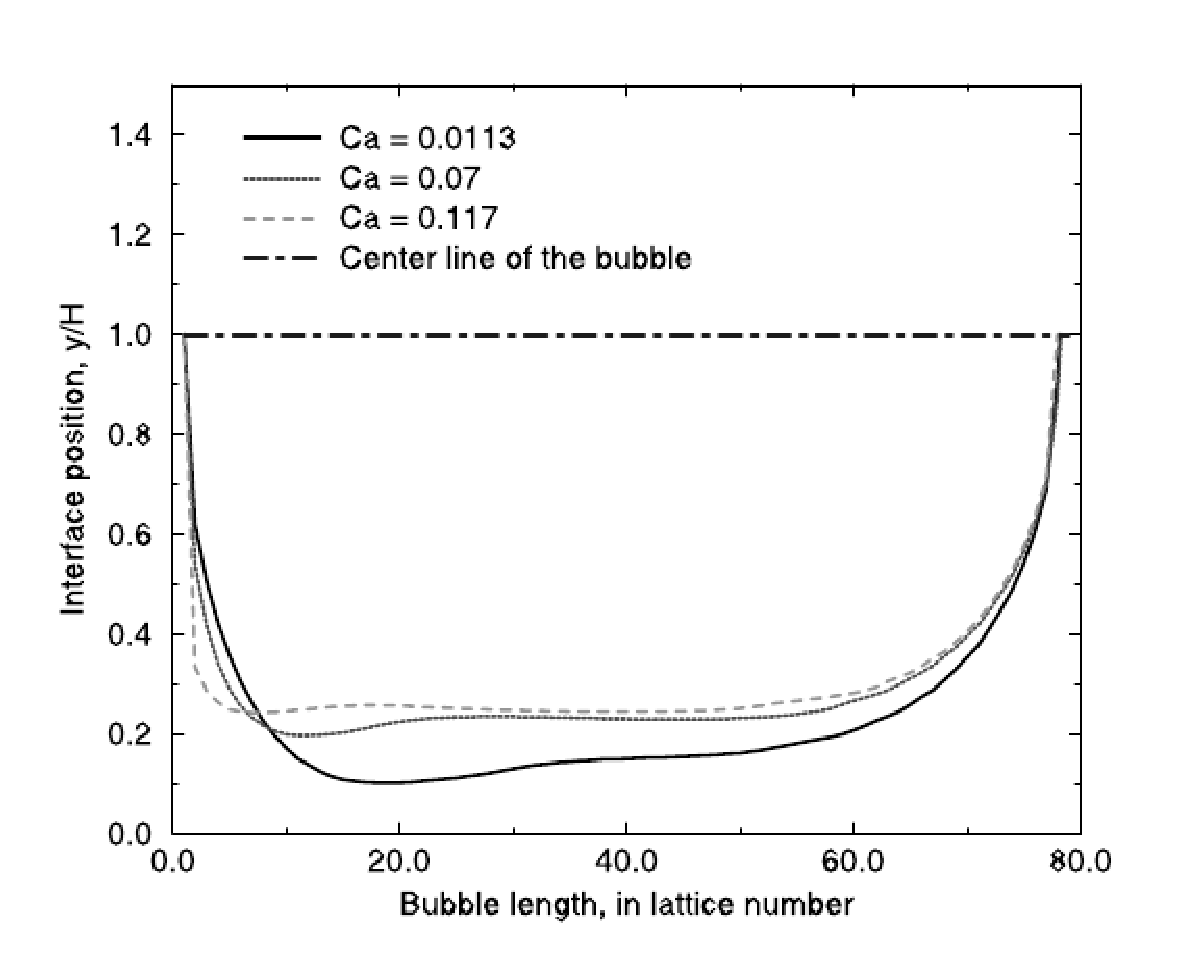
\includegraphics[width=0.47\textwidth]{Figures/Bubble/bubble_sehgal.eps}\\
\caption{The qualitative comparison for the film thickness across
the bubble length. Right (courtesy of \citet{sehgal-microchannel}),
left (present simulations).\label{fig:sehgal:bubble:length}}
\end{figure}
One can see a qualitative agreement, i.e. the thickness increases towards the front meniscus and
rapidly decreases towards the rear meniscus. This shape sometimes is called as a "bullet" shape.

\subsection{The influence of different viscosities}
The results obtained earlier are taken for the liquid viscosity ratio $10$.
We performed the same simulations for the liquid viscosity ratio of $20$.
The relaxation parameters were taken as $\tau_{\mathrm{liquid}}=4.5$ and $\tau_{\mathrm{bubble}}=0.7$. We
did not find any significant differences with the results obtained earlier. The
comparison for the liquid thicknesses is presented in Fig.
\ref{fig:capillary:viscous}. The results validate our assumption that in
the low capillary flow regime the density ratio does not affect the film thickness,
and that the gas-liquid viscosity ratio of the order $10$ is enough to obtain results
consistent with the Bretherton/Taylor problem.
\begin{figure}
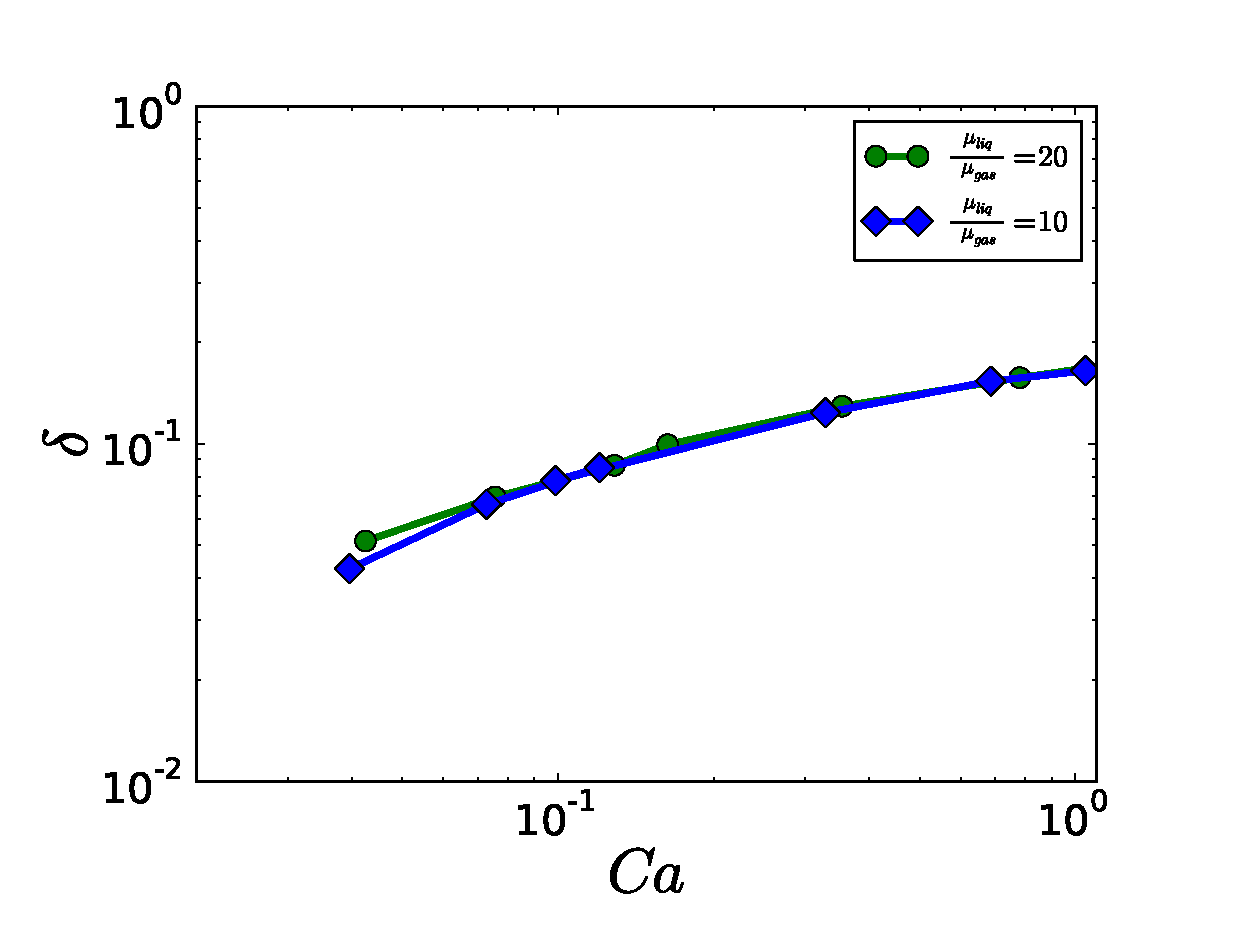
\includegraphics[width=0.97\textwidth]{Figures/Capillary_Viscous/capillaries_viscous.eps}
\caption{The film widths versus capillary number for
$\frac{\mu_{\mathrm{liq}}}{\mu_{\mathrm{gas}}}=10$ and $\frac{\mu_{\mathrm{liq}}}{\mu_{\mathrm{gas}}}=20$. The
results show good consistency and mutual agreement.\label{fig:capillary:viscous}}
\end{figure}

\section{Conclusion}
This work presents numerical tips and a benchmark for the
Bretherton/Taylor problem using the binary liquid lattice Botlzmann method. The
results show consistency with the previously published numerical results obtained
using other methods. Though our results are specific to the binary liquid lattice
Botlzmann method, the numerical hints and procedures can be used for any
continuous interface method.  We hope this work will prove to be valuable for
people simulating microchannel flows.

\bibliographystyle{plainnat}
\bibliography{paper}

\end{document}
